\chapter{Fieldwork data analysis}
Geological conditions are highly heterogeneous in the northern regions of Ghana. Subsurface characteristics vary at short mutual distance. Adequate and reliable local geohydrological information is preferably gathered by data collection through site-specific fieldwork. In this research perspective, multiple northern Ghana borehole locations are subjected to groundwater pumping tests. 
\bigskip \\
Spread over the Upper East and Northern Region the NGO Conservation Alliance (CA) holds several PIT locations, all originated in the summer of 2016. Four of these boreholes are by exception opened for the application of five pumping tests. A fifth PIT borehole (Ziong) has been made available for the monitoring of the ASR system-use by farmers. The figure below accommodates a map overview of the research locations within northern Ghana (Figure~\ref{fig:Overviewlocations}).
\bigskip 

\begin{figure}[ht]
 \centering
 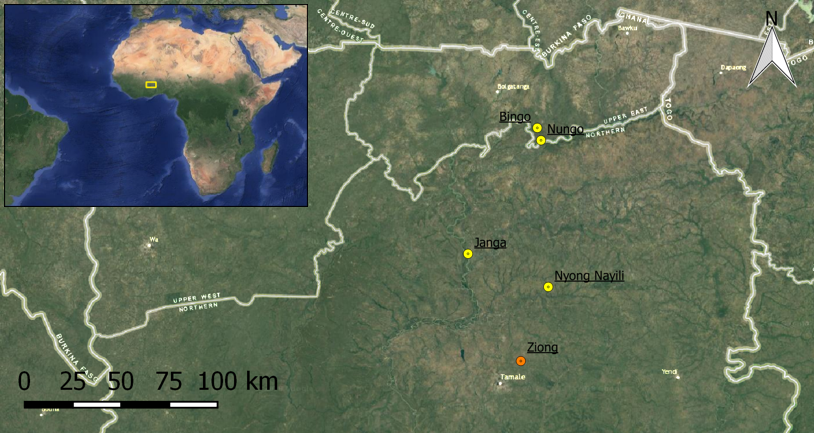
\includegraphics[width=\linewidth]{Overview_locations_northern_Ghana}
 \captionsetup{justification=centering} 
 \caption{Overview northern Ghana fieldwork locations}
 \label{fig:Overviewlocations}
\end{figure}

Detailed information on the used equipment and set-up of both the fieldwork pumping tests as well as the groundwater monitoring network (during daily ASR system-use) can be found in appendix \ref{chapter:fieldwork_set-up}. The obtained raw fieldwork data can be found in the site-specific fact-sheets of appendix \ref{section:fieldworkresults}. Gathered data acts as input in the derivation of the northern Ghana local geohydrological subsurface parameters; transmissivity (T) (hydraulic conductivity (k)) and storativity (S). 

This chapter accommodates the analysis and processing of gathered fieldwork data. First of all the (simplified) approach in data analysis, including the coherent theoretical background, is explained (section \ref{section:derivation_methods}). Section \ref{section:TS} contains the actual derivation of the site-specific groundwater parameter values: T and S. The chapter concludes with the determination of parameter bandwidths (section \ref{section:fieldwork_results}), applicable for the further purposes of this research; the model simulation and upscaling of northern Ghana ASR system-use. 

\section{Parameter derivation methods}
\label{section:derivation_methods}

\subsection{Theoretical model definition}
Large parts of the northern Ghana geohydrological soil characteristics are undiscovered. Strong variations in the geological conditions ensures the necessity of local knowledge in soil stratification. Most reliable site-specific information is recorded during borehole construction (2016). Content of the borehole log-sheets, available for the five research locations in appendix \ref{chapter:Borehole_logsheets}, is used as a starting point in the theoretical model determination. 
\\

Despite differences in present soil types, the research locations show similarities in stratification. In each case the soil top structure (approximately 50 m) is roughly divided into two or three layers (confining top layer). Groundwater tables are predominantly positioned in the first aquifer (layer under confining layer). Result is the selection of multiple (three in total) simplified theoretical models for the fieldwork data analysis, as depicted in figure \ref{fig:schematic_fieldwork_analysis}. 

\begin{figure}[h!]
	\centering
	\begin{subfigure}[b]{0.21\linewidth}
		\centering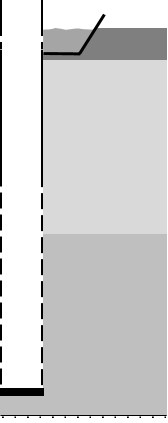
\includegraphics[width=0.6\linewidth]{Schematic_general_analysis}
		\captionsetup{justification=centering}		
		\caption{\label{fig:Schematic_general_analysis}}
		\end{subfigure}%\hfill
	\begin{subfigure}[b]{0.12\linewidth}
		\centering
\includegraphics[width=0.6\linewidth]{arrow_right}
		\end{subfigure}%\hfill
		%{\LARGE$\yrightarrow{}$}
	\begin{subfigure}[b]{0.21\linewidth}
		\centering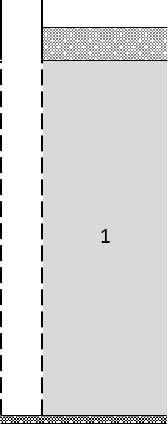
\includegraphics[width=0.6\linewidth]{Schematic_1lay_analysis}
		\captionsetup{justification=centering}		
		\caption{\label{fig:Schematic_1lay_analysis}}
		\end{subfigure}%\hfill
	\begin{subfigure}[b]{0.21\linewidth}
        \centering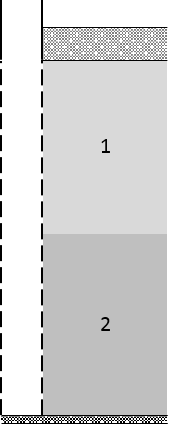
\includegraphics[width=0.6\linewidth]{Schematic_2lay_analysis}
		\captionsetup{justification=centering}		
		\caption{\label{fig:Schematic_2lay_analysis}}
		\end{subfigure}
	\begin{subfigure}[b]{0.21\linewidth}
        \centering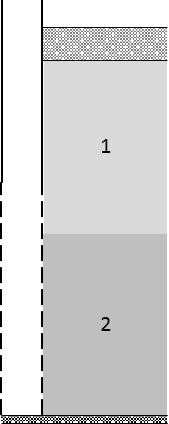
\includegraphics[width=0.6\linewidth]{Schematic_3lay_analysis}
		\captionsetup{justification=centering}		
		\caption{\label{fig:Schematic_3lay_analysis}}
		\end{subfigure}
	\captionsetup{justification=centering}	
	\caption{Schematic cross-sectional view of (\subref{fig:Schematic_general_analysis}) generalized northern Ghana soil stratification versus simplified (\subref{fig:Schematic_1lay_analysis}) single layered, ~(\subref{fig:Schematic_2lay_analysis}) double layered and ~(\subref{fig:Schematic_3lay_analysis}) partially penetrating double layered approaches in fieldwork data analysis} 
	\label{fig:schematic_fieldwork_analysis}
\end{figure} 

These simplified models (\ref{fig:Schematic_1lay_analysis} - \ref{fig:Schematic_3lay_analysis}) mimic local circumstances, making the derivation of representative hydraulic subsurface characteristics (T and S) possible (Kruseman \& de Ridder, 2000). Extension in the number of layers provides more degrees of freedom. Causing a double layered models to potentially simulate the gathered fieldwork data with higher accuracies. To limit chances of equifinality a maximum of two soil layers are implemented. \\ 

\subsection{Techniques in analysis}
\label{section:techniques_analysis}
Increased number of layers, and the degrees of freedom, suggest a gain in parameter derivation complexity. To enable the derivation of (multiple) hydraulic groundwater parameters, different suitable methods are applied. This section contains a detailed description of techniques applied. \\


\textbf{Analytical: Theis's method} \\ 
Groundwater drawdown due to the withdrawal of water can analytically be determined by Theis's equation (Equation \ref{eq:theis}). Theis's method is applicable on the situation depicted in \ref{fig:Schematic_1lay_analysis}; a constant rate pumping test in a fully penetrating well connected to a confined single layer aquifer (Kruseman \& de Ridder, 2000). The analytical solution is easily applicable and ideally suitable as a first geohydrological parameter indication.   

\begin{equation}
\label{eq:theis}
 s = \frac{Q}{4\pi K D} exp1(u)
\end{equation}

\begin{equation}
 u = \frac{r^{2} S}{4 K D t}
\end{equation}

Where s (m) is the drawdown at distance r (m) from the well, Q (m$^{3}$) is the constant well discharge , KD (m$^{2}$/d) is the aquifer transmissivity (KD = T), S (-) is the aquifer storativity, t (d) is the time measured from the start of pumping and exp1 is the exponential integral. The fieldwork drawdown measurements of this research are limited to in-well measurements only. For this research purposes the distance r in the Theis's equation is assumed to be the length of the well radius (0.0635 m). Theis's method is applicable for the time of pumping as well as the recovery process, as mentioned in the script below.\\

\begin{python}[h!]
def drawdown(t, T, S):
    s = Qo / (4 * np.pi * T) * exp1(ro ** 2 * S / (4 * T *t))
    s[t > toff] -= Qo / (4 * np.pi * T) * exp1(ro ** 2 * S / (4 * T *(t[t>toff] - toff)))   
    return s
\end{python}

\textbf{TTim Analytical Element modelling}\\
TTim is a computer program based on analytic elements and designed for the analysis of groundwater flow in one or more layers. The program is characterized by its simplistic model configuration. Multiple elements (and elements types) can be added one-by-one to specific predefined model layers. By the use of TTim (compared to the analytical Theis's method for example) it is possible to take additional well characteristics into account. Groundwater heads can be determined inside the well and the model optionally accounts for borehole storage and potential well skin resistance. Moreover, TTim is of particular functionality for the modelling of transient groundwater flow (bron??). Groundwater well discharge can be switched on and off easily and numerous times. Making TTim not only a program suitable for the simulation of a single pumping test(pumping and recovery), long duration use of the well can also be simulated. \\

The analysis of this fieldwork data is designed by the use of the TTim Model3D configuration. Although multiple elements can be part of the model, the inclusion of a single well (element) is sufficient in this case. Dependent on model design (\ref{fig:schematic_fieldwork_analysis}) the well (analytical element) is connected to one or more model layers. In the TTim fieldwork data analysis the model top layer configuration is tagged as confined with a true phreatic top (based on observed initial groundwater tables). By the use of this specific set-up the top layer storage coefficient (S) is a phreatic storage ($S_y$). Multiplying this value with the aquifer thickness is therefore no longer needed. This is moreover not an issue due to the general model simulation in which each model layer is defined with a 1 m thickness. The result is a simulation where derived hydraulic conductivities (K) can be interpreted as transmissivities (T) and the storage is expressed as the layer storage coefficient (S). This is predominantly done to directly derive T and S values. At the same time the approach naturally corrects for the unknown thickness of the deepest well penetrated soil layer (information on bottom soil layer depth absent in the borehole log-sheets of \ref{chapter:Borehole_logsheets}). \\

\textbf{MODFLOW}\\
The subsequent scenario modelling (chapter \ref{chapter:model_scenarios}) of this research is applied in USGS's modular model MODFLOW; the international standard in groundwater simulation (bron??). Regarding fieldwork data analysis MODFLOW is not used in the optimization process of geohydrological parameters. Optimal parameters (found by the use of TTim) are only implemented in corresponding MODFLOW simulations as a reference to validate the TTim results.

\subsection{Optimization functions}
Generated fieldwork pumping test data (section \ref{section:fieldwork_results}) is used as an input for the derivation of local geohydrological parameter values. The most likely applicable T and S values are determined by correlating the analytical solutions and/or TTim models to the gathered data. In this research optimization process two fit functions are applied. \\

\textbf{Fmin-RMSE optimization}\\
Deviations between fieldwork data and modelled drawdown curves can be expressed by the RMSE-value, equation \ref{eq:RMSE} (bron??). To minimize this error, and difference between modelled and fieldwork data, the Fmin function is applied (scipy.optimize package). Result is the determination of optimal T and S values (and optionally values for boreholes storage and well skin resistance) approximately representing the local circumstances. An example of Fmin-RMSE optimization python coding is depicted below. The example contains an optimization of five parameters (T and S values for two layers and an optimal well skin resistance). \\ 

\begin{equation}
\label{eq:RMSE}
 RMSE = \sqrt{\Sigma\frac{(s_{mod}-s_{field})^{2}}{N}}
\end{equation}

Where $s_{mod}$ is the modelled drawdown (m), $s_{field}$ is the fieldwork measured drawdown (m) and N is the number of data points. \\
 
\begin{python}[h!]
def optimTTim_Qvar(params, t, meas):
    kaq = np.zeros(2)
    Saq = np.zeros(2)
    kaq[0] = params[0]             
    kaq[1] = params[1]
    Saq[0] = params[2]
    Saq[1] = params[3]
    res = params[4]
    s = drawdownTTim_Qvar(t, kaq, Saq, res)
    error = np.sqrt(np.mean((s-meas)**2)) 
    return error

xopt = fmin(optimTTim_Qvar, x0=[10, 10, .01, .001, 0.1], args=(to[mask], do[mask]), xtol=1e-4)
\end{python}
\bigskip

\textbf{Calibration function}\\
Besides the application of minimizing the RMSE it is also possible to derive optimal geohydrological parameter values by the Calibrate function of TTim. This optimization function is applied in the research to improve the parameter value derivation robustness. In the python coding below, an example TTim Calibrate function is given. Content-wise it is the same example mentioned in the Fmin-RMSE optimization above.\\ 

\begin{python}[h!]
cal = Calibrate(mlc)
cal.parameter(name='kaq0', layer=0, initial=10, pmin=0)
cal.parameter(name='kaq1', layer=1, initial=10, pmin=0)
cal.parameter(name='Saq0', layer=0, initial=.01, pmin=0, pmax=0.3)
cal.parameter(name='Saq1', layer=1, initial=.001, pmin=0, pmax=0.3)
cal.parameter(name='res', par=wc.res, initial=0.1)
cal.series(name='obs3', x=ro, y=0, layer=[0,1], t=to[mask], h=-do[mask])
cal.fit()
\end{python}

These optimization techniques require initial parameter conditions. Possibly there is more than one optimal solution applicable. Making the outcome of the data analysis dependent on the arbitrary chosen starting values. Northern Ghana T and S values are commonly low (Owusu et al, 2017). In this  research the following initial conditions are applied: k$_{aq0}$ is 10 (m/d), k$_{aq1}$ is 10 (m/d), S$_{aq0}$ is 0.01 (-), S$_{aq1}$ is 0.001 (-) and well resistance is 0.1 (d). The in-field measured well radius is used as the (initial) borehole storage: 0.0635 (m). To avoid the occurrence of unlikely parameter values, boundary conditions are applied. The emergence of negative parameter values is prevented by setting the minimum parameter bound equal to zero. While unnaturally high storativity values are ignored by upper bounds of 0.3 (-).\

%(write something over initial conditions. Such small values. Not one single best solution. multiple 'best' solutions potentially close to each other. so solutions highly influential by the arbitrary chosen initial conditions. For each location several attempts done to see which initial conditions score pretty good. And subsequently generalization of those initial parameters applied per location/pumping test. for example better fit at Bingo at initial condition for T (KD) of 10, 10 (lay one and two) for fmin then for cal (2 layered system.) But 2 layered system all of sudden scores better with initial conditions 5, 1 for example.  

\section{From fieldwork data to T \& S values}
\label{section:TS}
Above mentioned model simplifications and methods in data analysis are applied on the research locations: Bingo, Nungo, Nyong Nayili, Janga and Ziong. In the TTim analsys an additional distinction is made by optionally applied optimizations in actual and/or optimal borehole storage and well resistance. A complete overview of all simulations applied can be found in appendix \ref{chapter:Extense_fieldwork_analaysis}. Most important outcomes of these analysis are for each research location further elaborated below.

\subsection{Location: Bingo}

\textbf{Site inspection}\\
Sloping landscape, some rocks at surface. Area dominated by bush fires, charred vegetation abundant, agricultural field not ready for use. Although Volta river not far (on map), no river, water flow or ponds seen in direct surroundings. Wet season floodings caused by rain and ’popping up’ out ground, labelled as heigh (1-2m) and disappears in days. At walking distance from nearest community. Steel lid, no tube perforations above surface level. \\

\textbf{Measurement quality}\\
Start delayed due to malfunctioning power converter. Tangled rope: Position lowest diver undesirably high and hand measurements not completely possible, result: big gab in data. Recovery test started at an early stage. \\

\textbf{Fit analysis} \\
Data point are missing. Total drawdown unknown from a certain moment in time. The analytical (Theis) solution is not capable of correcting for this measurement lack. This is most definitely not the case for the data analysed by the use of TTim. The use of both parameter optimization methods are capable of correcting for the lack of data. Both optimizations find optimal parameter values at which drawdown curve exceeds lowest measured groundwater levels. By this example it is shown it is not by definition required to feature complete drawdown curves during parameter determination. Even with incomplete drawdown time series it is possible to obtain reasonable fits. Complete overview of all the optimizations applied (13x) can be found in appendix.. tell about the wobbly curve, due to measured fluctuation in discharge. \\

\begin{figure}[h!]
 \centering
 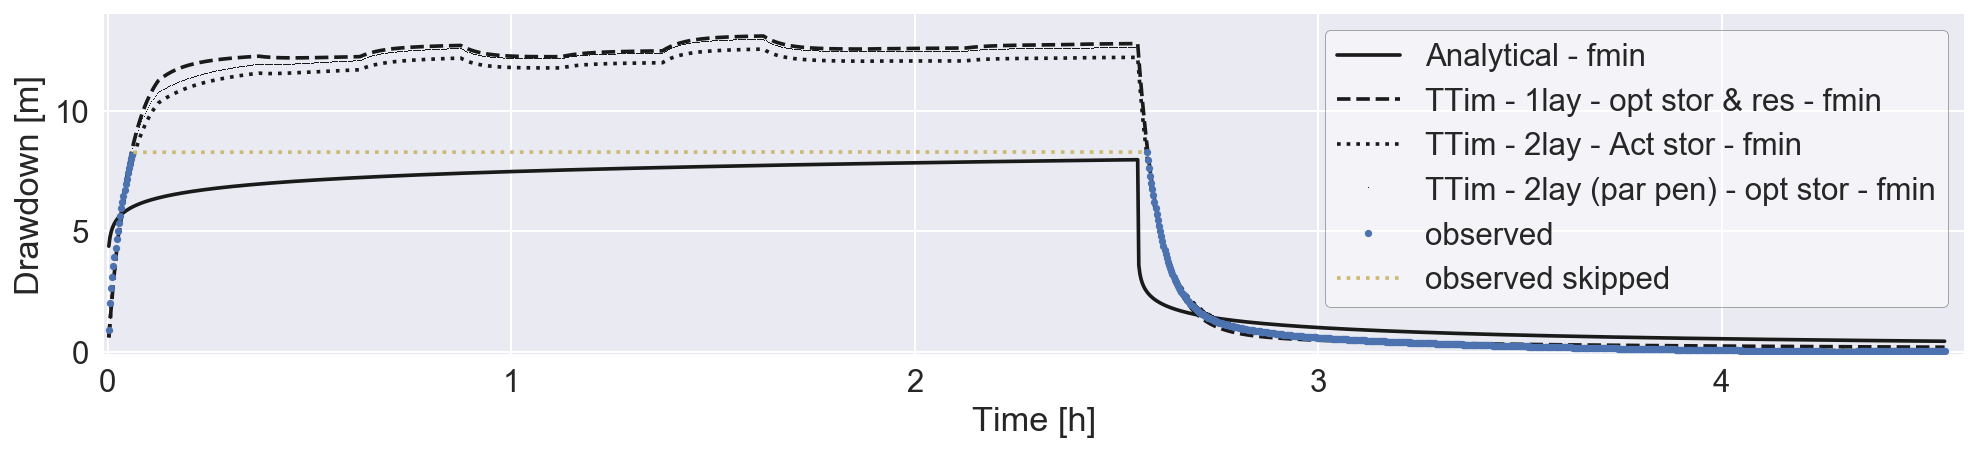
\includegraphics[width=\linewidth]{bingo_multi_lay_best}
 \captionsetup{justification=centering} 
 \caption{Bingo - multi-layer best fits}
 \label{fig:Bingo_best}
\end{figure}

\begin{table}[h!]
\small
\centering
\caption{Bingo - overview best fit parameters}
\label{tab:bing_table}
\begin{tabular}{l|l|l|l|ll|ll|l}
\hline 
\textbf{}       & \textbf{Method} & \textbf{Stor [m]} & \textbf{Res [d]} & \textbf{T1}  & \textbf{T2   [m$^2$/d]}  & \textbf{S1}  & \textbf{S2 [-]}  & \textbf{RMSE [m]} \\ \hline \hline
Analytical                & fmin             & -             & -            & 10.83      & -          & 2.0e-04    & -          & 0.798133 \\
1 lay                     & fmin             & 0.0647        & 5.6e-02      & 26.23      & -          & 6.6e-03    & -          & 0.162757 \\
2 lay                     & fmin             & 0.0635        & -            & 2.8e-04    & 08.25      & 3.0e-03    & 2.1e-06    & 0.107380 \\
2 lay (pp)                & fmin             & 0.0597        & -            & 8.6e-04    & 07.44      & 7.1e-03    & 6.3e-06    & 0.078188 \\ \hline    
\end{tabular}
\end{table}


%\begin{figure}[h!]
%	\centering
%	\begin{subfigure}[b]{1\linewidth}
%		\centering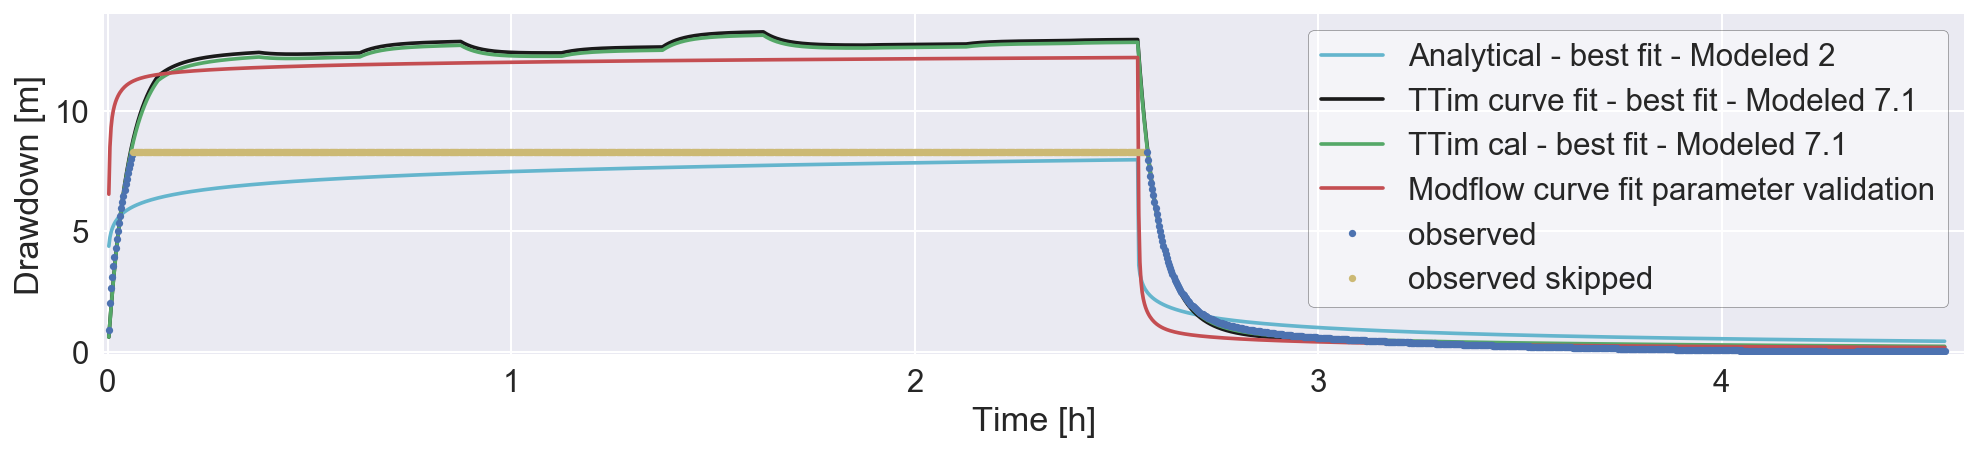
\includegraphics[width=1\linewidth]{bingo_1lay_analysis}
%		\captionsetup{justification=centering}		
%		\caption{\label{fig:bingo_1lay_analysis}}
%		\end{subfigure} \\ %\hfill
%	\begin{subfigure}[b]{1\linewidth}
%        \centering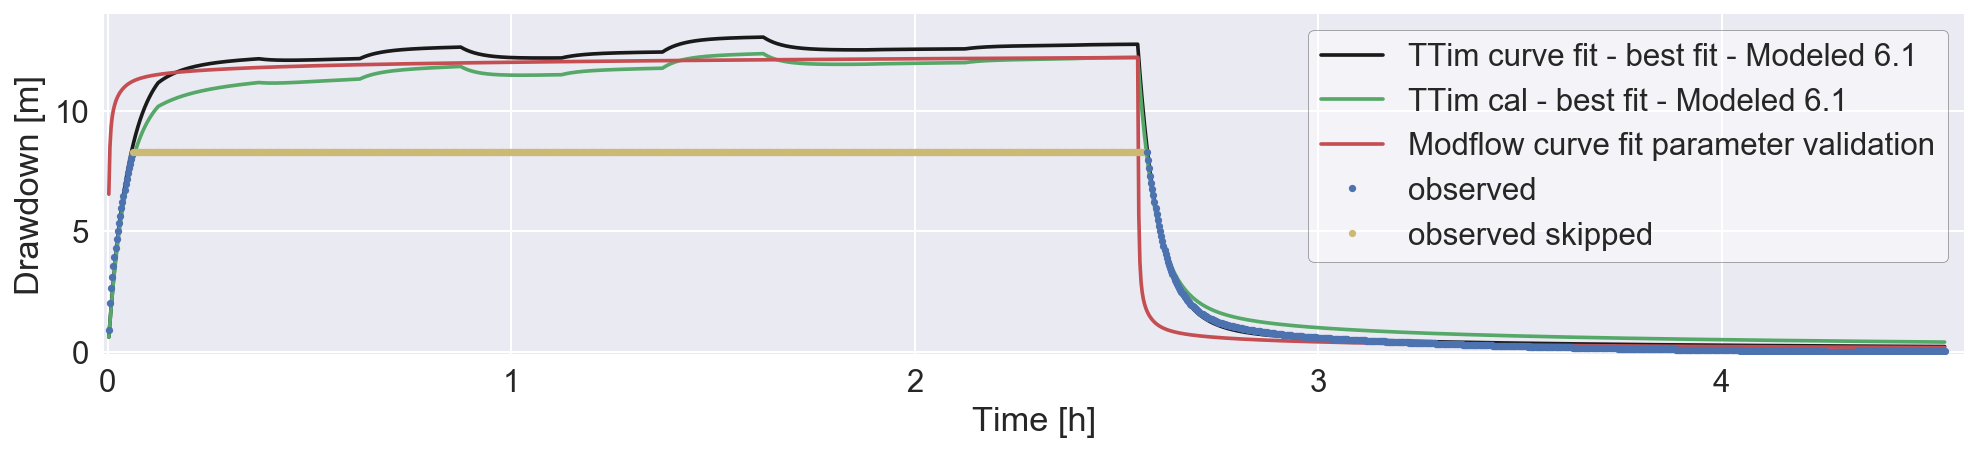
\includegraphics[width=1\linewidth]{bingo_2lay_analysis}
%		\captionsetup{justification=centering}		
%		\caption{\label{fig:bingo_2lay_analysis}}
%		\end{subfigure} \\
%	\begin{subfigure}[b]{1\linewidth}
%        \centering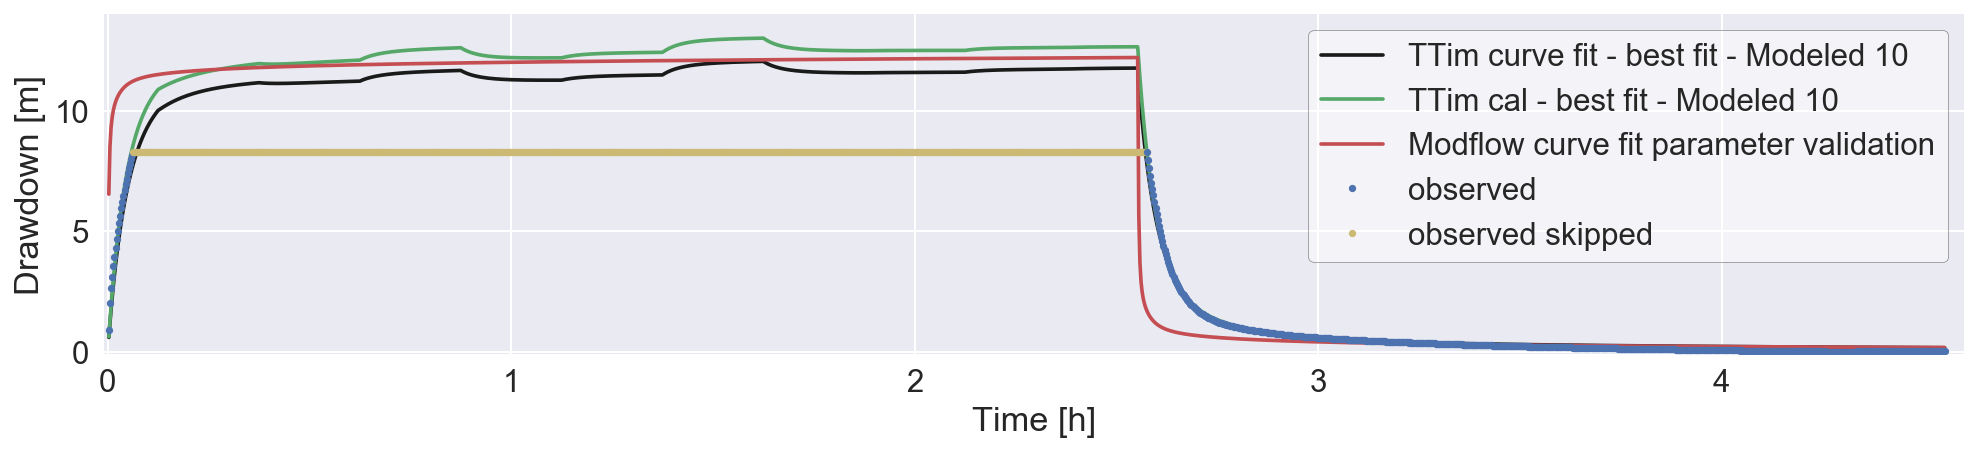
\includegraphics[width=1\linewidth]{bingo_3lay_analysis}
%		\captionsetup{justification=centering}		
%		\caption{\label{fig:bingo_3lay_analysis}}
%		\end{subfigure}
%	\captionsetup{justification=centering}	
%	\caption{Pumping test fit TS results: (\subref{fig:bingo_1lay_analysis}) single layered, ~(\subref{fig:bingo_2lay_analysis}) double layered and ~(\subref{fig:bingo_3lay_analysis}) triple layered (partially penetrating)} 
%	\label{fig:bingo_fieldwork_analysis}
%\end{figure} 

%
%\begin{table}[h!]
%\small
%\centering
%\caption{Bingo - overview best fit parameters}
%\label{tab:bingo_table}
%\begin{tabular}{l|l|l|lll|lll|l}
%\hline 
%\textbf{}       & \textbf{Stor [m]} & \textbf{Res [d]} & \textbf{T1}& \textbf{T2}  & \textbf{T3   [m$^2$/d]}  & \textbf{S1}& \textbf{S2}  & \textbf{S3 [-]}  & \textbf{RMSE [m]} \\ \hline
%\textbf{Single Lay}       & \textbf{} & \textbf{} & \textbf{}& \textbf{}& \textbf{}  & \textbf{}& \textbf{}& \textbf{}  & \textbf{}                    \\ \hline
%Analytical                & -             & -            & 10.83      & -          & -          & 2.0E-04    & -          & -          & 0.798         \\
%Curve fit                 & -             & 0.05         & 25.52      & -          & -          & 7.3E-05    & -          & -          & 0.166         \\
%Cal                       & -             & 2.5E-04      & 21.94      & -          & -          & 5.9E-19    & -          & -          & 0.175         \\
%{\textbf{}}               &               &              &            &            &            &            &            &            &               \\ 
%\textbf{Double Lay}       & \textbf{} & \textbf{} & \textbf{}& \textbf{}& \textbf{}  & \textbf{}& \textbf{}& \textbf{}  & \textbf{}                    \\ \hline
%Curve fit                 & -             & 0.06         & 22.88      & 0.40       & -          & 4.2E-04    & 8.0E-04    & -          & 0.167         \\
%Cal                       & -             & 0.02         & 11.63      & 0.57       & -          & 3.3E-07    & 4.7E-06    & -          & 0.413         \\ {\textbf{}}               &               &              &            &            &            &            &            &            &               \\ 
%\textbf{Triple Lay}       & \textbf{} & \textbf{} & \textbf{}& \textbf{}& \textbf{}& \textbf{}& \textbf{}& \textbf{}& \textbf{}                        \\ \hline
%Curve fit                 & -             & -            & 6.28       & 1.6E-03    & 0.86       & 1.8E-06    & 1.7E-02    & 2.0E-03    & 0.163         \\
%Cal                       & -             & -            & 17.95      & 3.76       & 3.35       & 0.18167    & 0.29988    & 0.11243    & 0.076         \\ \hline    
%\end{tabular}
%\end{table}


\textbf{Final remark}
korte uitleg welke fit nou het beste is? en waarom. 

\subsection{Location: Nungo}

\textbf{Site inspection}

\textbf{Measurement quality}

\textbf{Fit analysis}

\textbf{Final remark}

\subsection{Location: Nyong Nayili}


\textbf{Site inspection}

\textbf{Measurement quality}
data skip applied. 
\textbf{Fit analysis}

\begin{figure}[h!]
 \centering
 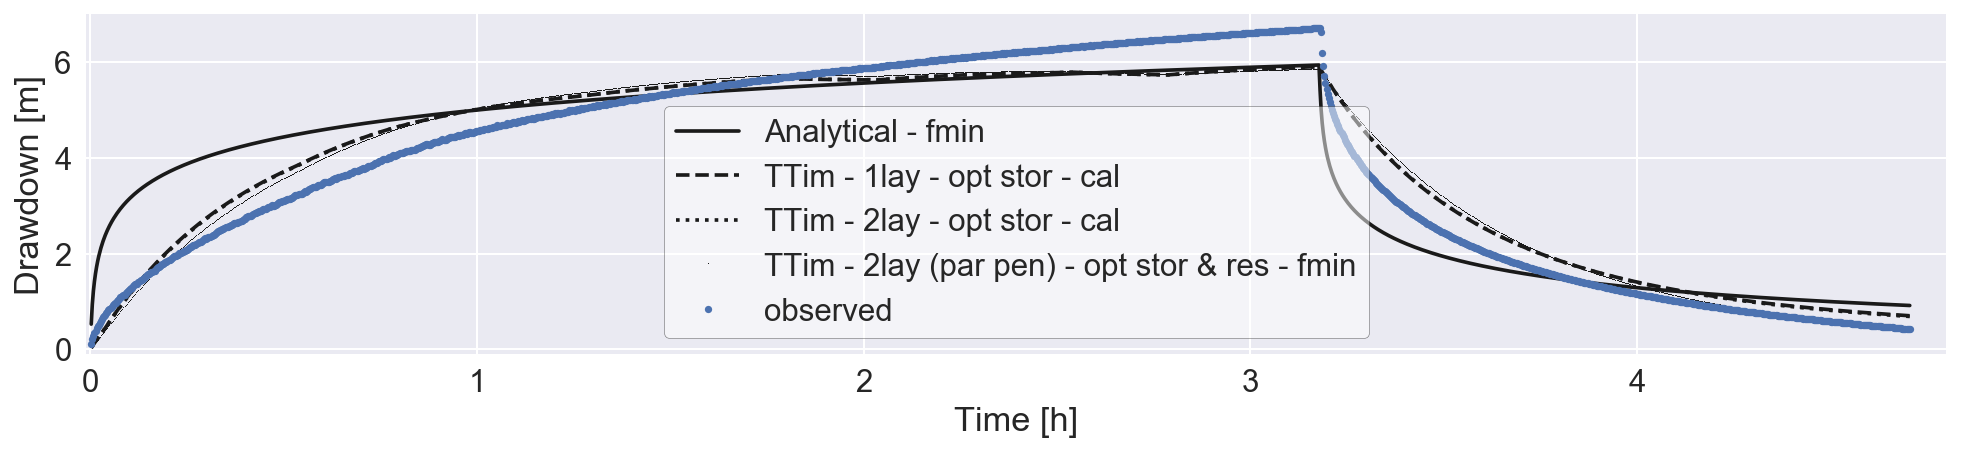
\includegraphics[width=\linewidth]{Nyong_Nayili_multi_lay_best}
 \captionsetup{justification=centering} 
 \caption{Nyong Nayili - multi-layer best fits}
 \label{fig:Nyong_Nayili_best}
\end{figure}

\begin{table}[h!]
\small
\centering
\caption{Nyong Nayili - overview best fit parameters}
\label{tab:Nyong_Nayili_table}
\begin{tabular}{l|l|l|l|ll|ll|l}
\hline 
\textbf{}       & \textbf{Method} & \textbf{Stor [m]} & \textbf{Res [d]} & \textbf{T1}  & \textbf{T2   [m$^2$/d]}  & \textbf{S1}  & \textbf{S2 [-]}  & \textbf{RMSE [m]} \\ \hline \hline
Analytical                & fmin             & -             & -            & 06.00      & -          & 3.0e-01    & -          & 0.751699 \\
1 lay                     & cal              & 0.2419        & -            & 13.35      & -          & 7.8e-05    & -          & 0.457474 \\
2 lay                     & cal              & 0.2436        & -            & 06.95      & 06.98      & 4.6e-06    & 3.6e-05    & 0.456774 \\
2 lay (pp)                & fmin             & 0.2659        & 1.7e-02      & 1.7e-04    & 28.61      & 1.1e-02    & 4.4e-06    & 0.450121 \\ \hline    
\end{tabular}
\end{table}


\textbf{Final remark}


\subsection{Location: Janga (1/2)}

\textbf{Site inspection}

\textbf{Measurement quality}

\textbf{Fit analysis}

\begin{figure}[h!]
 \centering
 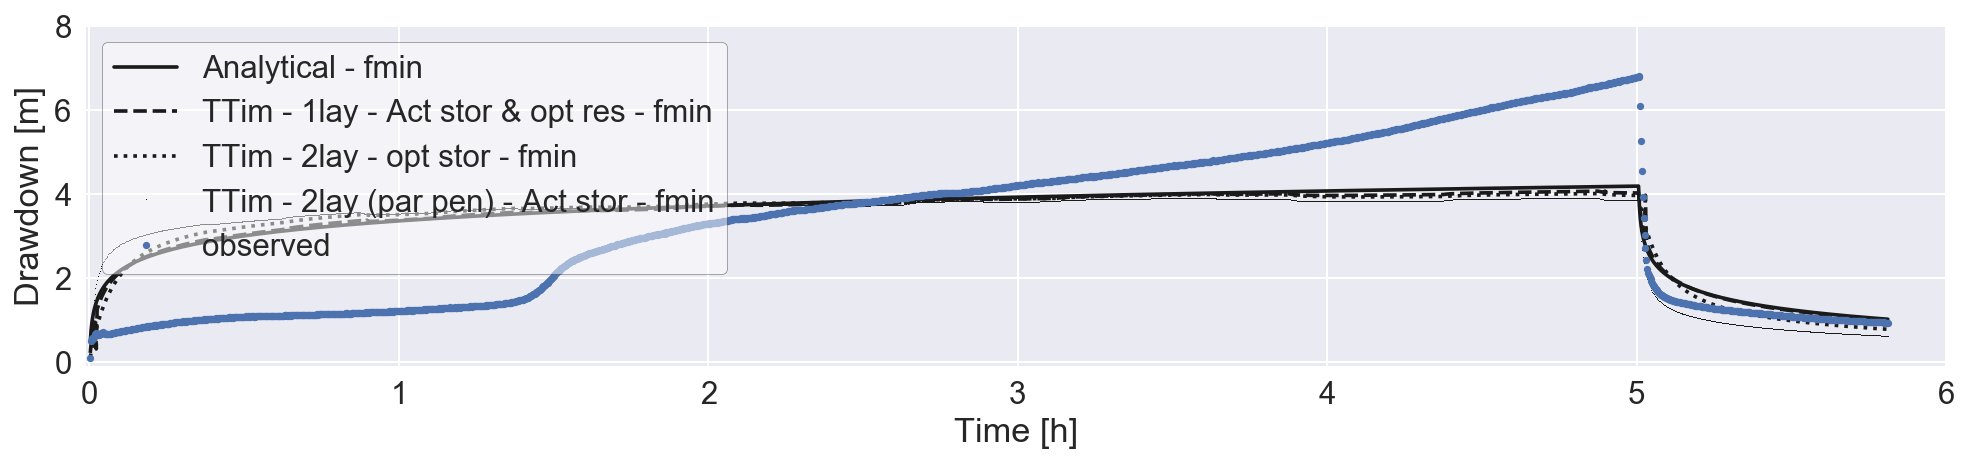
\includegraphics[width=\linewidth]{Janga1_multi_lay_best}
 \captionsetup{justification=centering} 
 \caption{Janga first attempt - multi-layer best fits}
 \label{fig:Janga1_best}
\end{figure}

\begin{table}[h!]
\small
\centering
\caption{Janga first attempt - overview best fit parameters}
\label{tab:Janga1_table}
\begin{tabular}{l|l|l|l|ll|ll|l}
\hline 
\textbf{}       & \textbf{Method} & \textbf{Stor [m]} & \textbf{Res [d]} & \textbf{T1}  & \textbf{T2   [m$^2$/d]}  & \textbf{S1}  & \textbf{S2 [-]}  & \textbf{RMSE [m]} \\ \hline \hline
Analytical                & fmin             & -             & -            & 08.84      & -          & 3.0e-01    & -          & 1.338604 \\
1 lay                     & fmin             & 0.0635        & -9.7e-03     & 09.09      & -          & 1.6e-02    & -          & 1.382181 \\
2 lay                     & fmin             & 0.1287        & -            & 12.48      & 1.3e-04    & 1.9e-02    & 1.1e-08    & 1.444546 \\
2 lay (pp)                & fmin             & 0.0635        & -            & 9.1e-05    & 15.19      & 4.3e-08    & 3.1e-03    & 1.530254 \\ \hline    
\end{tabular}
\end{table}

\textbf{Final remark}

\subsection{Location: Janga (2/2)}

\textbf{Measurement quality}

\textbf{Fit analysis}

\begin{figure}[h!]
 \centering
 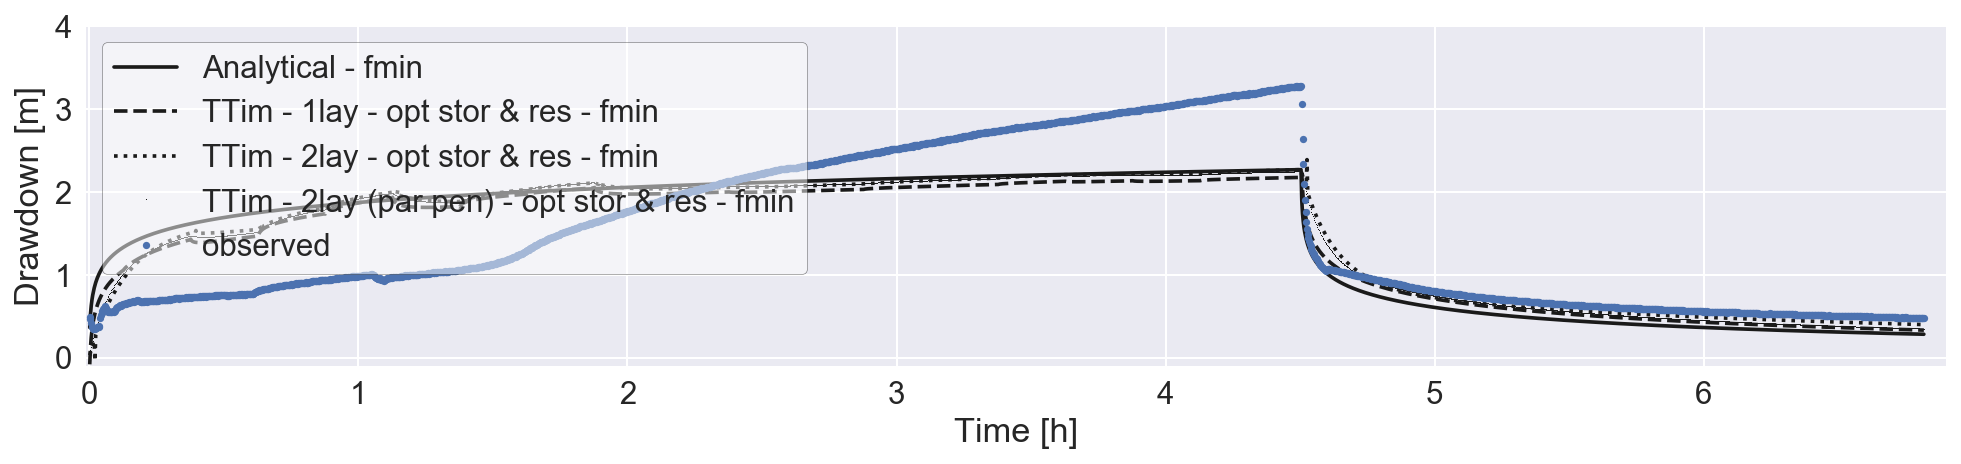
\includegraphics[width=\linewidth]{Janga2_multi_lay_best}
 \captionsetup{justification=centering} 
 \caption{Janga second attempt - multi-layer best fits}
 \label{fig:Janga2_best}
\end{figure}

\begin{table}[h!]
\small
\centering
\caption{Janga second attempt - overview best fit parameters}
\label{tab:Janga2_table}
\begin{tabular}{l|l|l|l|ll|ll|l}
\hline 
\textbf{}       & \textbf{Method} & \textbf{Stor [m]} & \textbf{Res [d]} & \textbf{T1}  & \textbf{T2   [m$^2$/d]}  & \textbf{S1}  & \textbf{S2 [-]}  & \textbf{RMSE [m]} \\ \hline \hline
Analytical                & fmin             & -             & -            & 15.97      & -          & 3.0e-01    & -          & 0.570855 \\
1 lay                     & fmin             & 5.4e-07       & -9.7e-03     & 13.54      & -          & 1.9e-02    & -          & 0.550853 \\
2 lay                     & fmin             & 0.2228        & -2.2e-02     & 02.05      & 08.13      & 2.1e-02    & 4.1e-04    & 0.544680 \\
2 lay (pp)                & fmin             & 0.2005        & -3.1e-02     & 06.59      & 00.86      & 9.4e-05    & 2.1e-03    & 0.544540 \\ \hline    
\end{tabular}
\end{table}

\textbf{Final remark}

\subsection{Location: Ziong (monitoring)}


\textbf{Site inspection}

\textbf{Measurement quality}
multi day use. Anaytical solution not applied. 
\textbf{Fit analysis}

\begin{figure}[h!]
 \centering
 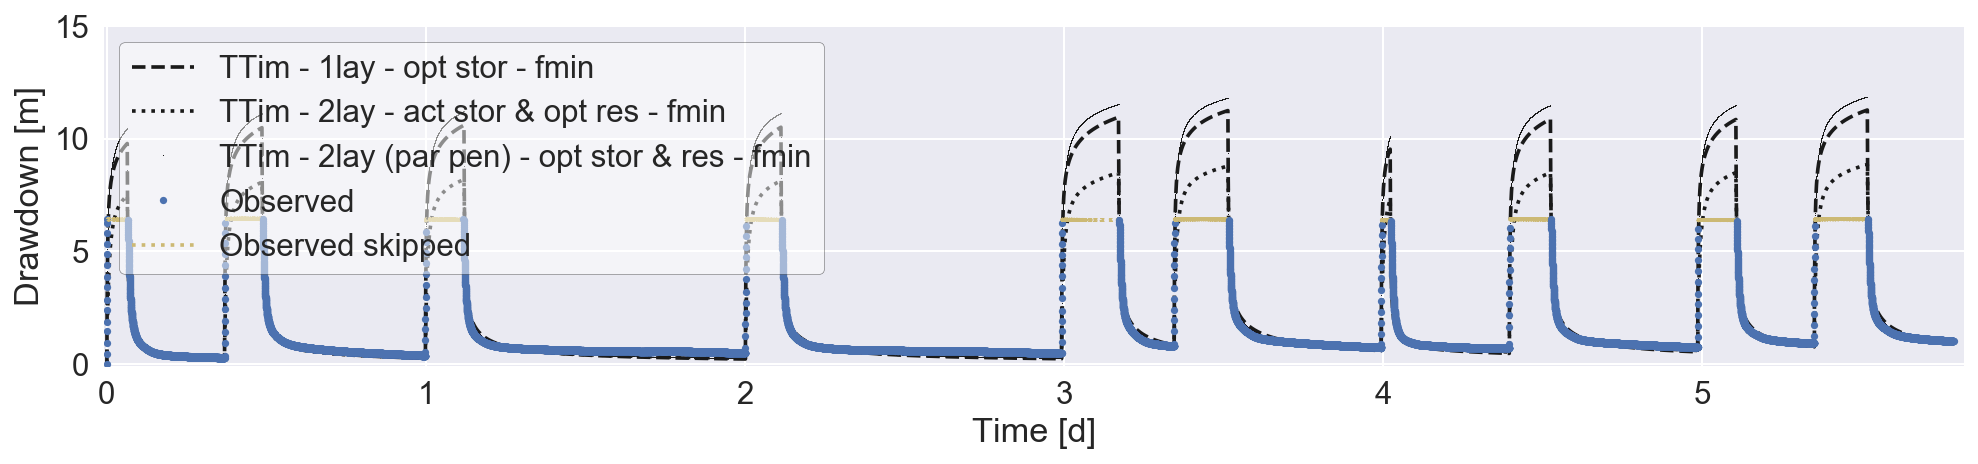
\includegraphics[width=\linewidth]{Ziong_multi_lay_best}
 \captionsetup{justification=centering} 
 \caption{Ziong - multi-layer best fits}
 \label{fig:Ziong_best}
\end{figure}

\begin{table}[h!]
\small
\centering
\caption{Ziong - overview best fit parameters}
\label{tab:Ziong_table}
\begin{tabular}{l|l|l|l|ll|ll|l}
\hline 
\textbf{}       & \textbf{Method} & \textbf{Stor [m]} & \textbf{Res [d]} & \textbf{T1}  & \textbf{T2   [m$^2$/d]}  & \textbf{S1}  & \textbf{S2 [-]}  & \textbf{RMSE [m]} \\ \hline \hline
1 lay                     & fmin             & 0.0382        & -            & 01.76      & -          & 1.1e-03    & -          & 0.254574 \\
2 lay                     & fmin             & 0.0635        & -0.05        & 00.38      & 01.05      & 2.9e-02    & 1.2e-03    & 0.240162 \\
2 lay (pp)                & fmin             & 0.0147        & -0.08        & 00.23      & 00.78      & 2.6e-02    & 1.3e-03    & 0.243108 \\ \hline    
\end{tabular}
\end{table}

\textbf{Final remark}

\section{Theoretical validation}

\textbf{Soil analysis}

\textbf{VES analysis}


\section{Fieldwork results}
\label{section:fieldwork_results}

summary of the main results
Recommendations for further investigation if applicable. 

Waardes komen overeen (zelfde range/ordegrootte) met theorie. zoek dit even na \\

Er is geen duidelijk onderscheid of 1, 2 dan wel 3 laags (partially penetrating) beter dan wel slechter scoort. dus alle schematische gelaagde bodemoppbouw mogelijk. \\ 

bespreek hier de tekortkoming van het meten in de well zelf als enige. Werkt gewoon niet heel fijn of nauwkeurig. Voor indicatie wel goed. \\ 

vertel over het resultaat van de twee vormen van analyse. fmin versus calibration function. Toch een verschil in alhoritme (numerieke solver). Maar resultaten beide slechts tot op zekere hoogte nauwkeurig. Maar dit zal eerder komen door de metingen zelf (in borehole) en de omstansigheden van northern Ghana. \\ 

does not happen to often. but if T or S values not in right 'order', it is alsways assumed highest T values in layer under confining layer (not in lowest layer). based on the known soil ype of this layer in borehole logsheet (appendiox..). \\

schrijf appendix over de lambda bepaling. 